\documentclass[man]{apa7}
\usepackage[]{graphicx}\usepackage[]{color}
% maxwidth is the original width if it is less than linewidth
% otherwise use linewidth (to make sure the graphics do not exceed the margin)
\makeatletter
\def\maxwidth{ %
  \ifdim\Gin@nat@width>\linewidth
    \linewidth
  \else
    \Gin@nat@width
  \fi
}
\makeatother

\definecolor{fgcolor}{rgb}{0.345, 0.345, 0.345}
\newcommand{\hlnum}[1]{\textcolor[rgb]{0.686,0.059,0.569}{#1}}%
\newcommand{\hlstr}[1]{\textcolor[rgb]{0.192,0.494,0.8}{#1}}%
\newcommand{\hlcom}[1]{\textcolor[rgb]{0.678,0.584,0.686}{\textit{#1}}}%
\newcommand{\hlopt}[1]{\textcolor[rgb]{0,0,0}{#1}}%
\newcommand{\hlstd}[1]{\textcolor[rgb]{0.345,0.345,0.345}{#1}}%
\newcommand{\hlkwa}[1]{\textcolor[rgb]{0.161,0.373,0.58}{\textbf{#1}}}%
\newcommand{\hlkwb}[1]{\textcolor[rgb]{0.69,0.353,0.396}{#1}}%
\newcommand{\hlkwc}[1]{\textcolor[rgb]{0.333,0.667,0.333}{#1}}%
\newcommand{\hlkwd}[1]{\textcolor[rgb]{0.737,0.353,0.396}{\textbf{#1}}}%
\let\hlipl\hlkwb

\usepackage{framed}
\makeatletter
\newenvironment{kframe}{%
 \def\at@end@of@kframe{}%
 \ifinner\ifhmode%
  \def\at@end@of@kframe{\end{minipage}}%
  \begin{minipage}{\columnwidth}%
 \fi\fi%
 \def\FrameCommand##1{\hskip\@totalleftmargin \hskip-\fboxsep
 \colorbox{shadecolor}{##1}\hskip-\fboxsep
     % There is no \\@totalrightmargin, so:
     \hskip-\linewidth \hskip-\@totalleftmargin \hskip\columnwidth}%
 \MakeFramed {\advance\hsize-\width
   \@totalleftmargin\z@ \linewidth\hsize
   \@setminipage}}%
 {\par\unskip\endMakeFramed%
 \at@end@of@kframe}
\makeatother

\definecolor{shadecolor}{rgb}{.97, .97, .97}
\definecolor{messagecolor}{rgb}{0, 0, 0}
\definecolor{warningcolor}{rgb}{1, 0, 1}
\definecolor{errorcolor}{rgb}{1, 0, 0}
\newenvironment{knitrout}{}{} % an empty environment to be redefined in TeX

\usepackage{alltt}
\usepackage{graphicx}
%% for inline R code: if the inline code is not correctly parsed, you will see a message
\newcommand{\rinline}[1]{SOMETHING WRONG WITH knitr}

\IfFileExists{upquote.sty}{\usepackage{upquote}}{}
\usepackage[american]{babel}
\usepackage{mathtools}
\usepackage{hyperref}
\usepackage[american]{babel}
\usepackage{csquotes}
\usepackage[style=apa,sortcites=true,sorting=nyt,backend=biber]{biblatex}
\DeclareLanguageMapping{american}{american-apa}
\addbibresource{/media/jeksterslab/scripts/r/jeksterslabRdoc/inst/extdata/bib.bib}
\title{Sample Asciidoctor/LaTeX Document Using Jekdoc Tags}
\twoauthors{Ivan Jacob Agaloos Pesigan}{John H. Doe}
\twoaffiliations{University of Macau}{University of Macau}
\leftheader{Pesigan & Doe}
\authornote{
\addORCIDlink{Ivan Jacob Agaloos Pesigan}{0000-0003-4818-8420}
\href{mailto:i.j.a.pesigan@connect.um.edu.mo}{i.j.a.pesigan@connect.um.edu.mo}
Department of Psychology,
University of Macau;
\addORCIDlink{John H. Doe}{0000-0000-0000-0000}
\href{mailto:johndoe@email.com}{johndoe@email.com}
Department of Psychology,
University of Macau

Correspondence concerning this article should be addressed to
Ivan Jacob Agaloos Pesigan,
Department of Psychology, Faculty of Social Sciences, Avenida da Universidade, University of Macau, Taipa, Macau SAR, China.
Email: \href{mailto:i.j.a.pesigan@connect.um.edu.mo}{i.j.a.pesigan@connect.um.edu.mo}
}
\abstract{This document demonstrates how to use \texttt{Jekdoc tags}. This document covers the following: headers, text styling, Math, R code, citations, tables and others. The following is a boilerplate text with \texttt{Jekdoc tags}. Lorem ipsum dolor sit amet \textcite{Anderson04}, consectetur adipiscing elit, sed do eiusmod tempor incididunt ut labore et dolore magna aliqua. Ut enim ad minim veniam, quis nostrud exercitation ullamco laboris nisi ut aliquip ex ea commodo consequat \textcite{Lane12a, Lane12b}. \textbf{\emph{This is bold italic text.}} Duis aute irure dolor in reprehenderit in voluptate velit esse cillum dolore eu fugiat nulla pariatur. Excepteur sint occaecat cupidatat non proident, sunt in culpa qui officia deserunt mollit anim id est laborum. \textbf{This is bold text.} \emph{This is italic text.} \enquote{This is text in double quote.} \enquote*{This is text in single quote.} This is an example of text with\textsubscript{superscript}. This is an example of text with\textsuperscript{subscript}. \texttt{This is monospace text.} This is an inline Math equation with \texttt{R} code $\pi = rinline{pi}$.}

\keywords{Jekdoc, Asciidoc, Latex}
\begin{document}
\maketitle

\section{Headers}

\section{Header 1}

\subsection{Header 2}

\subsubsection{Header 3}

\paragraph{Header 4}

\subparagraph{Header 5}

\section{Text Styling}

Lorem ipsum dolor sit amet, consectetur adipiscing elit, sed do eiusmod tempor incididunt ut labore et dolore magna aliqua. Ut enim ad minim veniam, quis nostrud exercitation ullamco laboris nisi ut aliquip ex ea commodo consequat. \textbf{\emph{This is bold italic text.}} Duis aute irure dolor in reprehenderit in voluptate velit esse cillum dolore eu fugiat nulla pariatur. Excepteur sint occaecat cupidatat non proident, sunt in culpa qui officia deserunt mollit anim id est laborum. \textbf{This is bold text.} \emph{This is italic text.} \enquote{This is text in double quote.} \enquote*{This is text in single quote.} This is an example of text with\textsubscript{superscript}. This is an example of text with\textsuperscript{subscript}. \texttt{This is monospace text.}

Accented \`{e}

\section{Math}

\subsection{Inline equation}

This is an inline equation: $\Sigma = \Sigma \left( \theta \right)$.

\subsection{Centered equation}

\begin{equation}
\label{eq}
c^2 = a^2 + b^2
\end{equation}

This is a reference to Equation \ref{eq}.

\section{R}

\subsection{Inline}

The following are examples of inline \texttt{R} code.

Lorem ipsum dolor sit amet,
consectetur adipiscing elit,
sed do eiusmod tempor incididunt ut labore et dolore magna aliqua. rinline{x <- c(5, 4, 6, 7); x}.

Ut enim ad minim veniam, rinline{mean(x)},
quis nostrud exercitation ullamco laboris nisi ut aliquip ex ea commodo consequat.

\subsection{R code chunk}

The following are examples of \texttt{R} chunks.

\begin{knitrout}
\definecolor{shadecolor}{rgb}{0.969, 0.969, 0.969}\color{fgcolor}\begin{kframe}
\begin{alltt}
\hlnum{1}\hlopt{+}\hlnum{1}
\end{alltt}
\begin{verbatim}
## [1] 2
\end{verbatim}
\begin{alltt}
\hlkwd{rnorm}\hlstd{(}\hlnum{5}\hlstd{)}
\end{alltt}
\begin{verbatim}
## [1]  0.9021226 -1.3030961  1.3528918 -1.2342237 -1.3264467
\end{verbatim}
\begin{alltt}
\hlnum{1}\hlopt{:}\hlnum{2}\hlopt{+}\hlnum{1}\hlopt{:}\hlnum{3} \hlcom{# a warning}
\end{alltt}

{\ttfamily\noindent\color{warningcolor}{\#\# Warning in 1:2 + 1:3: longer object length is not a multiple of shorter object length}}\begin{verbatim}
## [1] 2 4 4
\end{verbatim}
\begin{alltt}
\hlstd{f}\hlkwb{=}\hlkwa{function}\hlstd{()\{}\hlkwd{message}\hlstd{(}\hlstr{'Aloha, this is a friendly message!'}\hlstd{)\}}
\hlkwd{f}\hlstd{()}
\end{alltt}

{\ttfamily\noindent\itshape\color{messagecolor}{\#\# Aloha, this is a friendly message!}}\begin{alltt}
\hlnum{1}\hlopt{+}\hlstr{'a'} \hlcom{# mision impossible}
\end{alltt}

{\ttfamily\noindent\bfseries\color{errorcolor}{\#\# Error in 1 + "{}a"{}: non-numeric argument to binary operator}}\end{kframe}
\end{knitrout}

\begin{knitrout}
\definecolor{shadecolor}{rgb}{0.969, 0.969, 0.969}\color{fgcolor}\begin{kframe}
\begin{alltt}
\hlkwd{par}\hlstd{(}\hlkwc{mar}\hlstd{=}\hlkwd{c}\hlstd{(}\hlnum{4}\hlstd{,} \hlnum{4}\hlstd{,} \hlnum{.1}\hlstd{,} \hlnum{.1}\hlstd{))}
\hlkwd{plot}\hlstd{(cars,} \hlkwc{pch}\hlstd{=}\hlnum{19}\hlstd{)}
\end{alltt}
\end{kframe}\begin{figure}
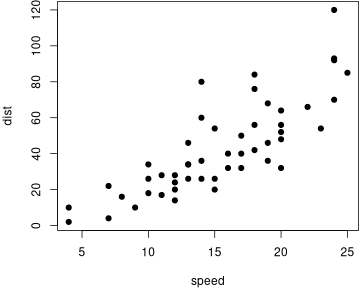
\includegraphics[width=\maxwidth]{/home/jek/test/cool-plot-1} \caption[A wonderful plot]{A wonderful plot.}\label{fig:cool-plot}
\end{figure}

\end{knitrout}

\section{Citations}

\textcite{Anderson04} (citet, single)

\textcite{Lane12a, Lane12b} (citet, multiple)

\textcite*{Anderson04} (citet*, single)

\textcite*{Lane12a, Lane12b} (citet*, multiple)

\cite{Anderson04} (citealt, single)

\cite{Lane12a, Lane12b} (citealt, multiple)

\cite*{Anderson04} (citealt*, single)

\cite*{Lane12a, Lane12b} (citealt*, multiple)

\parencite{Anderson04} (citep, single)

\parencite{Lane12a, Lane12b} (citep, multiple)

\parencite*{Anderson04} (citep*, single)

\parencite*{Lane12a, Lane12b} (citep*, multiple)

\cite{Anderson04} (citealp, single)

\cite{Lane12a, Lane12b} (citealp, multiple)

\cite*{Anderson04} (citealp*, single)

\cite*{Lane12a, Lane12b} (citealp*, multiple)

\citeauthor{Anderson04} (citeauthor, single)

\citeauthor{Lane12a, Lane12b} (citeauthor, multiple)

\citeauthor*{Anderson04} (citeauthor*, single)

\citeauthor*{Lane12a, Lane12b} (citeauthor*, multiple)

\citeyear{Anderson04} (citeyear, single)

\citeyear{Lane12a, Lane12b} (citeyear, multiple)

\citeyear{Anderson04} (citeyearpar, single)

\citeyear{Lane12a, Lane12b} (citeyearpar, multiple)

\fullcite{Anderson04} (fullcite)

\section{Comment}

%% kjkjklsjgjhbjnjglksjgkjsgf

\section{Others}

\noindent{} No indent text.

\printbibliography

\appendix
\end{document}
